\lfoot{Autor: Daniel Melichar}
\subsubsection{Relationale Datenbanken}
\label{subsec:relationaleDB}

Die relationale Datenbank ist seit dem ersten Erscheinen in den 1970er Jahren weit gekommen und ist von den meisten Großkonzernen der Welt adaptiert worden \cite{MELD.CH2-relationaleDB.ranking}. Mit der eigens dafür entwickelten Abfragesprache SQL \textit{(Structured Query Langauge)} war das Umgehen mit Datenbanken und Tabellen und der darin gespeicherten Information so einfach wie noch nie.

\begin{figure}[!htb]\centering
	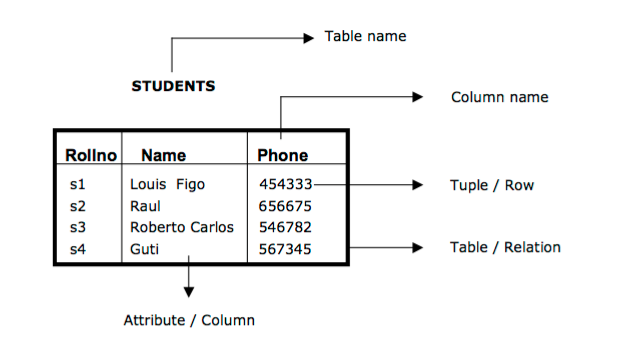
\includegraphics[width=0.8\textwidth]{images/relationaleTabelle}
	\caption{Beispiel einer relationalen Tabelle}
\end{figure}

Features von relationalen DBMS (Achtung: diese sind stark vom eigentlichem DBMS abhängig)
\begin{itemize}
\item Unterstützten eine große Menge an Daten
\item Datensicherheit durch Authentifizierung, Permissions, etc.
\item Fehlertoleranz und Wiederherstellung
\end{itemize}

Hinter den Kulissen sorgt das Relational Database Management System (RDBMS) dafür, dass die Eigenschaften des ACID Prinzips (Atomicity, Consistency, Isolation, Durability) eingehalten werden. Für eine detailierte Beschreibung zum ACID Prinzip, siehe Sektion \ref{subsec:acidvsbase}. Features der Abrfagsprache SQL, so wie Constraints (primary and foreign keys, Datentype, etc.) oder Stored Procedures/Functions, sorgen dafür, dass ein RDBMS die beste Performance bei simplen Abfragen von mittelgroßen Datemengen hat \cite{MELD.CH2-relationaleDB.performacne}.

Einige der größten Limitierungen \cite{MELD.CH2-relationaleDB.rdbmsBuch} durch das relationale Datenbankmodel sind
\begin{itemize}
\item Skalierbarkeit: Bei komplexen Abfragen in großen Datenbanken sind RDBMS im Vergleich langsamer \cite{MELD.CH2-relationaleDB.performacne}.
\item Komplexität: die Daten müssen zu Tabellen strukturiert werden; es ist also ein Schema notwendig
\item Abfragesprache: Obwohl SQL ein ANSI (American National Standards Institute) Standard ist, gibt es verschiedene Versionen der Sprache. Es müssen aber alle Hauptfunktionen (wie SELECT, UPDATE, DELETE, INSERT, WHERE) gegeben sein, um den ANSI Standard zu erfüllen.
\end{itemize}

Die Verwendung eines relationalen Datenbankmanagementsystemes macht also dann Sinn, wenn ein Datenschema erstellt werden kann, also wenn bekannt ist, welche konkreten Daten gesammelt werden und wie diese in Tabellen mit Beziehungen verarbeitet werden können. Durch die SQL Abfragesprache bekommt der Datenbank-Administrator alle Features, die er braucht, um das System in Takt zu halten.